\documentclass[11pt]{memoir}

\usepackage{mathtools}
\usepackage{physics}
\usepackage{tikz}

\begin{document}

\begin{equation*}
    f(x) = \sum_{n=0}^\infty \frac{(x-a)^n}{n!}\eval{\dv[n]{f}{x}}_{x=a}
\end{equation*}

$x \rightarrow x+h$ $a=x$

\begin{align*}
    f(x+h) &= \sum_{n=0}^\infty \frac{(x + h - x)^n}{n!}\eval{\dv[n]{f}{(x+h)}}_{(x+h)=x}\\
    &= \sum_{n=0}^\infty \frac{h^n}{n!}\eval{\dv[n]{f}{(x+h)}}_{(x+h)=x}\\
    &= \sum_{n=0}^\infty \frac{h^n}{n!}\eval{\dv[n]{f}{x}}_{x=x}
\end{align*}

\begin{align*}
    \dv{f}{(x+h)} &= \dv{f}{x}\dv{x}{(x+h)} = \dv{f}{x}\qty(\dv{(x+h)}{x})^{-1}\\ &= \dv{f}{x}\qty(\dv{x}{x} + \dv{h}{x})^{-1} = \dv{f}{x}\qty(1 + 0)^{-1}\\
    &= \dv{f}{x}
\end{align*}

Udledning af eulers metode ud fra taylor ekspansion for $n=1$:

\begin{align*}
    f(x+h) &\approx \sum_{n=0}^1 \frac{h^n}{n!}\eval{\dv[n]{f}{x}}_{x=x}\\
    &\approx \frac{h^0}{0!}\eval{\dv[0]{f}{x}}_{x=x} + \frac{h^1}{1!}\eval{\dv[1]{f}{x}}_{x=x}\\
    &\approx f(x) + h\dv{f}{x}
\end{align*}

Udledning af eulers metode ud fra differensligning:
\begin{equation*}
    \dv{f}{x} = g(x,f(x))
\end{equation*}
\begin{align*}
    \dv{f}{x} &= \lim_{h \rightarrow 0}\qty(\frac{f(x+h) - f(x)}{h})\\
    \dv{f}{x} &\approx \frac{f(x+h) - f(x)}{h}
\end{align*}
\begin{equation*}
    f(x+h) \approx f(x) + hg(x,f(x))
\end{equation*}

\tikzset{axes/.style={->,>=stealth}}
\tikzset{vector/.style={->,>=stealth}}

\begin{tikzpicture}
\draw[->] (0,-0.2) -- (0,3);
\draw[->] (-0.2,0) -- (5,0);
\draw plot [smooth] coordinates {(0,2) (1.5,1) (3,2.75) (4.5,1)};
\end{tikzpicture}

\begin{tikzpicture}[scale=3.5,domain=0:1.25,smooth,declare function={fcnf(\x) =-\x^2+1.5*\x; fcng(\x)=-0.25*sin(deg((\x-0.15)*5))+0.3;}]

\def\a{0.19}
\def\b{0.978}

\path (-0.2,0) node(xline){} (1.5,0);
\path (0,-0.2) node(yline){} (0,1.5);

\fill[green!10]  plot[domain=\a:\b] (\x,{fcnf(\x)}) -- plot[domain=\b:\a] (\x,{fcng(\x)});
\draw plot (\x,{fcnf(\x)}) node[right] {$f(x)$};
\draw plot (\x,{fcng(\x)}) node[right] {$g(x)$};

\draw[dashed] (\a,{fcnf(\a)}) -- ({(\a,fcnf(\a))} |- xline) node[below]{$a$};
\draw[dashed] (\b,{fcng(\b)}) -- ({(\b,fcng(\b))} |- xline) node[below]{$b$};

%{-0.25*sin({deg({(0.987-0.15)}*5)})+0.3}

\draw[axes] (-0.2,0) -- (1.5,0) node[right] {$x$};
\draw[axes] (0,-0.2) -- (0,1.5) node[above] {$y$};

\end{tikzpicture}


\begin{tikzpicture}[scale=3.5,domain=0:1.25,smooth,declare function={fcnf(\x) =-\x^2+1.5*\x; fcng(\x)=-0.25*\x*sin(deg((\x-0.15)*5))+0.5;}]

\def\a{0.22}
\def\b{0.978}
\def\h{0.25}

\path (-0.2,0) node(xline){} (1.5,0);
\path (0,-0.2) node(yline){} (0,1.5);

%\fill[green!10]  plot[domain=\a:\b] (\x,{fcnf(\x)}) -- plot[domain=\b:\a] (\x,{fcng(\x)});


%\foreach \n in {1,2,3,4,5}{
%\fill[green!200]  plot[domain=\h*(\n-1):\h*\n] (\x,{fcng(\x)}) -- ({\n*\h}, 0) -- ({\h*(\n-1)}, 0) -- (\h*(\n-1),{fcng(\h*(\n-1))});}
%\filldraw[green!200, draw=black,style=dashed]  ({\h*\n},{fcng(\h*\n)}) -- ({\n*\h}, 0) -- ({\h*\n-\h}, 0) -- (\h*\n-\h,{fcng(\h*\n-\h)});}
%\foreach \n in {1,2,3,4,5}{
%\draw[dashed] (\n*\h,{fcng(\n*\h)}) -- ({(\n*\h,fcng(\n*\h))} |- xline) node[below]{$b$};}
\draw plot (\x,{fcng(\x)}) node[right] {$g(x)$};

\draw[axes] (-0.2,0) -- (1.5,0) node[right] {$x$};
\draw[axes] (0,-0.2) -- (0,1.5) node[above] {$y$};

\end{tikzpicture}

kjhgkj
\begin{tikzpicture}[scale=0.5,domain=0:6,smooth,declare function={fcnf(\x) =-\x^2+1.5*\x; fcng(\x)=0.25*\x^3-\x^2+3;}]

\def\a{0.22}
\def\b{0.978}
\def\h{0.25}

\path (-0.2,0) node(xline){} (12,0);
\path (0,-0.2) node(yline){} (0,20);


\draw plot (\x,{fcng(\x)}) node[right] {$g(x)$};

\draw[axes] (-0.2,0) -- (12,0) node[right] {$x$};
\draw[axes] (0,-0.2) -- (0,20) node[above] {$y$};
\end{tikzpicture}

lkhjlkjh

\usetikzlibrary{decorations.pathreplacing}

\vspace{1cm}
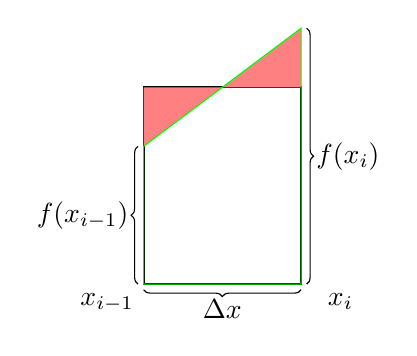
\begin{tikzpicture}
\draw[thick] (0,0) rectangle (2,2.5);
%\draw (0,2.5) ;
\draw (2.5,0) node[below]{$x_{i}$};

\fill[red!50] (0,1.75) -- (2,3.25) -- (2,2.5) -- (0,2.5) -- cycle;

\draw[green, decoration={brace}] (0,0) node[below left, black]{$x_{i-1}$}  -- (0,1.75) -- (2,3.25)  -- (2,0) -- cycle;

\draw[decoration={brace}, xshift=-2pt, decorate] (0,0) -- node[left]{$f(x_{i-1})$} (0,1.75);

\draw[decoration={brace, mirror}, xshift=2pt, decorate] (2,0) -- node[right]{$f(x_{i})$} (2, 3.25);

\draw[decoration={brace, mirror}, yshift=-2pt, decorate] (0,0) -- node[below]{$\Delta x$} (2,0);


\end{tikzpicture}



\end{document}